\capitulo{5}{Aspectos relevantes del desarrollo del proyecto}

El planteamiento de este proyecto ha ido variando durante su desarrollo. Al ser un proyecto de investigación y aprendizaje, el objetivo de este también ha ido evolucionando.
El primer paso del desarrollo del proyecto consistió en hacer una investigación y pruebas de concepto. Se hizo una investigación de qué herramientas podrían ser mejores para el desarrollo de este proyecto.

\section{Java}
La primera prueba de concepto consistió en la elaboración del juego sin motor gráfico, haciéndolo desde cero con el IDE eclipse usando java. El objetivo de la prueba de concepto era conseguir elaborar una pequeña pantalla que imprimiese un laberinto con el algoritmo más sencillo posible. 

El primer paso fue ver cuál podría ser la forma más sencilla de implementar, y se encontró el laberinto de Wilson, aunque no es la forma más eficiente de generar laberintos de mayor tamaño.

Tras esto comenzó el desarrollo de la prueba de concepto, pero no había demasiada documentación online y era muy costoso de realizar por lo que no se terminó la prueba y se descartó.

\section{C\# y .NET}
La segunda prueba de concepto fue desarrollada en C\#, este lenguaje no era la primera opción ya que se carecía de experiencia con él, pero resultó ser muy parecido a java por lo que la curva de aprendizaje fue más suave. Desarrollarlo en .NET tiene como gran desventaja que a la hora de escalarlo y hacer mazmorras, es muy limitante. Hace que resulte muy costoso dibujar el mapa, por lo que esta opción fue también descartada antes de terminar la prueba de concepto.

\section{Unity - Primera fase}
La tercera prueba de concepto se realizó de una forma mucho más cómoda que las dos anteriores. Al ser un motor de videojuegos, tiene una comunidad mucho mayor, lo que ayudó en el desarrollo de esta misma. La prueba de concepto consigue lograr el objetivo y con muy poco código tener el generador de laberintos funcionando.

Esta primera fase del proyecto tenía como objetivo que dibujase en 2D un laberinto y que este fuese jugable.
La parte principal, consiste en una matriz en la que vamos a ir alterando con un algoritmo si hay o no una pared, y esto lo iríamos dibujando por toda la matriz. 

\begin{algorithm}
\caption{GenerarLaberinto}
\begin{algorithmic}
\Procedure{GenerarLaberinto}{tamañoX, tamañoY}
    \State laberinto = nuevo arreglo bidimensional de enteros con tamaño (tamañoX, tamañoY)
    \State entero maxX = obtenerLímiteSuperior(laberinto, 0)
    \State entero maxY = obtenerLímiteSuperior(laberinto, 1)
    
    \For{entero i desde 0 hasta tamañoX}
        \For{entero j desde 0 hasta tamañoY}
            \If{i == 0 o j == 0 o i == maxX o j == maxY}
                \State laberinto[i][j] = 1
            \Else
                \If{i es par y j es par}
                    \If{valorAleatorio() > umbralColocación}
                        \State laberinto[i][j] = 1
                        \State entero a, b
                        \If{valorAleatorio() < 0.5}
                            \State a = 0
                        \Else
                            \If{valorAleatorio() < 0.5}
                                \State a = -1
                            \Else
                                \State a = 1
                            \EndIf
                        \EndIf
                        \If{a != 0}
                            \State b = 0
                        \ElsIf{valorAleatorio() < 0.5}
                            \State b = -1
                        \Else
                            \State b = 1
                        \EndIf
                        \State laberinto[i + a][j + b] = 1
                    \EndIf
                \EndIf
            \EndIf
        \EndFor
    \EndFor
\EndProcedure
\end{algorithmic}
\end{algorithm}

En el pseudocódigo de \emph{Algorithm 1} se puede observar que tiene ciertas características y estructuras algorítmicas que son similares a las que se utilizan en el <<Laberinto de Wilson>>, un algoritmo de generación de laberintos que funciona eligiendo un punto de inicio aleatorio y extiende caminos desde él hasta que se conecta con un camino existente. No es idéntico, pero comparte la idea de crear caminos aleatorios dentro de un área determinada.

El laberinto resultante tenía el aspecto de la figura \ref{fig:PrimerLaberinto}.
\begin{figure}[hb]  
    \centering  
    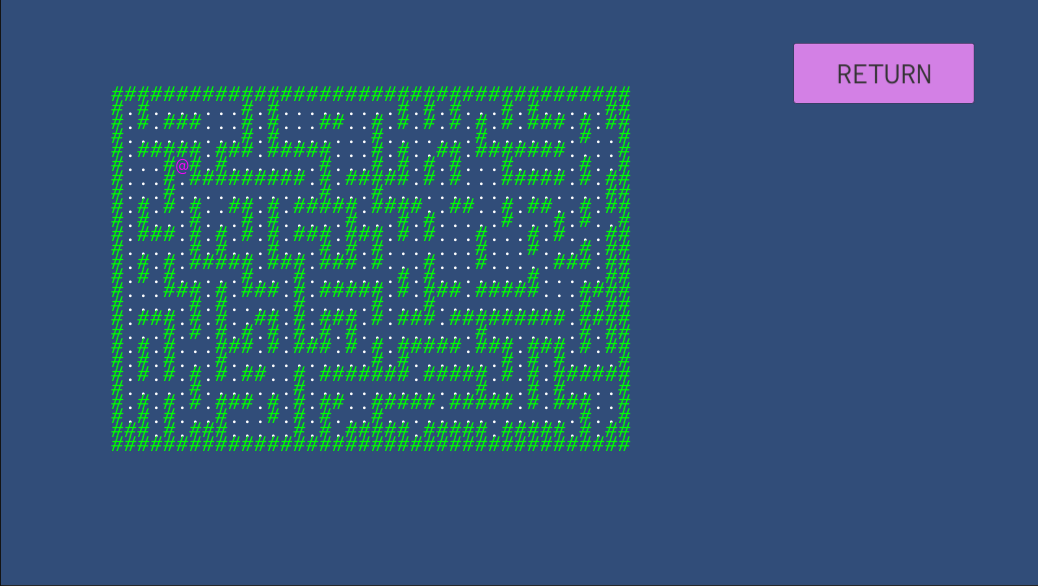
\includegraphics[width=\textwidth]{img/PrimerLaberinto.png}  
    \caption{Primer laberinto generado en Unity.}  
    \label{fig:PrimerLaberinto}
\end{figure}

Cuando se renderiza o <<dibuja>> el mapa con el jugador (representado por el icono @), cada vez que este icono se movía, internamente en Unity se obligaba a dibujar el mapa al completo. Esto es muy ineficiente, para solucionar este problema, en la siguiente iteración, ya se comienza a hacer uso del objeto que Unity proporciona, \texttt{GameObject}.

Un \texttt{gameObjects}~\cite{UnityGameObject} es la unidad básica de organización y representación en una escena, es similar a un objeto en java. En este caso convertir al jugador en un \texttt{gameObjects} nos quitará la necesidad de ir dibujando constantemente el mapa, y entran en juego las animaciones en tiempo real que realiza el motor.

Tras comenzar a refactorizar el proyecto de Unity, se llegó a la conclusión de que era mucho más eficiente empezar un proyecto desde cero, por ello se creó la carpeta <<SegundaFase>>, en esta se realizaría el proyecto de una forma más organizada. Habría consumido mucho más tiempo intentar refactorizar todo el proyecto anterior.


\section{Unity - Segunda fase}
En esta segunda fase, el proyecto a desarrollar cambia por completo. Ahora el proyecto va a imitar la arquitectura cliente - servidor que se emplea en la industria, el servidor va a enviar al cliente, en este caso Unity, lo que tiene que dibujar.

\subsection{Preparación del back-end}
Las primeras semanas fueron para investigar cómo construir este servidor y cual sería la forma más sencilla de hacerlo. 
\subsubsection{Construcción de la API}
Para \textbf{construir la API}, la elección fue FastAPI, ya que al ser tan popular, hay mucha documentación, haciendo la curva de aprendizaje más suave. Una de las grandes ventajas de FastAPI es su documentación automática, desde la que se puede testear la API directamente, sin necesidad de desarrollar interfaz gráfica. Esto hizo los primeros pasos muy dinámicos, ya que el esfuerzo se podía centrar en desarrollar el servidor y los algoritmos.

\subsubsection{Preparación de los algoritmos}
Los \textbf{algoritmos} se desarrollaron en Python, y el servidor se va a encargar de generarlos, almacenarlos y enviar el resultado en forma de JSON al cliente. Este luego se encargará de leer y dibujar en el motor para que sean jugables. 

Muchos de los algoritmos primero fueron desarrollados en un Notebook de Jupyter en paralelo, así se facilita el desarrollo sin necesidad de tener que ir probando con Unity para ver cómo se dibujan. Cuando ya se tenía el algoritmo funcional, se necesitó ir adaptando ya que al principio no se estaba teniendo en cuenta la semilla para la generación de estos laberintos.

\subsubsection{Preparación de la base de datos}

Para poder \textbf{almacenar información} en la base de datos al principio se pensó que la mejor opción era SQLite, y se comenzó a desarrollar. 
SQLite, que es SQL, tiene la desventaja de que utiliza un modelo relacional con tablas y esquemas rígidos, y esto quita una flexibilidad muy necesaria cuando se decidió cambiar el modelo de datos. 

Un cambio importante en el almacenamiento de los laberintos surgió cuando se pensó en que era más óptimo almacenar los laberintos al completo, junto con su \textbf{semilla}. Esto se debe a que la generación procedimental es determinista, es decir, que con las mismas entradas se produce la misma salida, por ello es tan eficiente y útil almacenar la semilla.

Para hacer esto se cambió a una base de datos \textbf{NoSQL}, está orientada a documentos que almacena datos en formato BSON. Esto ofrece mucha más flexibilidad, haciendo que los datos no estén semi-estructurados, así si los datos cambian con el tiempo se puede adaptar. Este cambio nace por la inmediatez que ofrece al acceder a los laberintos y que desaparece la necesidad de establecer relaciones entre entidades. MongoDB ofrece replicación y tolerancia a fallos haciendo que los datos estén disponibles incluso en caso de problemas de hardware o red.


\subsection{Preparación del juego}
Para poder usar Unity como cliente, una parte clave ha sido \textbf{UnityWebRequest}, esta clase permite realizar llamadas HTTP, pudiendo así conseguir llamar al servidor con el algoritmo que seleccionado y para que devuelva el laberinto generado. 
Cuando Unity recibe el .JSON, lo transforma y con la matriz resultante que ha enviado el servidor, lo dibuja.

En Unity para este proyecto se han creado varios scripts, tanto para el control del <<Menu>> y de las pantallas como para poder dibujar en el motor y navegar el mapa. 

Gracias al sistema de físicas que tiene Unity por defecto, ha sido mucho más sencillo desarrollar el juego, utilizando mallas (Mesh~\cite{unitymesh}). Una malla consiste en una gran cantidad de triángulos y vértices que definen la forma de un objeto tridimensional, almacenados en un array, esta malla se podría poner rodeando al objeto 3D deseado y hacer que se comporte como material físico. Esto es lo que va a rodear a los cubos que van a interactuar como paredes para el jugador, de lo contrario el jugador podría atravesar el laberinto. Esto va a ir programado en un script que luego se va a cargar en el <<GameManager>>, el objeto que va estar encargado de cargar los scripts asociados.

Para que la cámara no se quede estancada y pueda seguir al jugador, hace falta un script que vaya a tiempo real con el jugador. Para ello hizo falta encontrar la rotación adecuada. Fue una tarea de prueba y error, hasta que se decidió no rotar la cámara porque se perdía visibilidad de la bola.

El evento para que cargue la escena hace también la llamada al servidor, entre escenas no se almacena la información, por lo que para poder guardar lo que el usuario haya seleccionado y se pueda enviar en la llamada, fue clave el uso de <<PlayerPreferences>>~\cite{unityplayerprefs}, es una clase de Unity que en la que se puede cargar la información y aunque se cambie de escena esta información no se pierde, por lo que se puede volver a cargar en las escenas que se necesiten.

